\documentclass[11pt]{article}
\usepackage{amsmath}
\usepackage{amssymb}
\usepackage{graphicx}
\usepackage{tabularx}
\usepackage{fancyhdr}
\usepackage{lastpage}

% Page layout
\usepackage[top=1in, bottom=1in, left=1in, right=1in]{geometry}

% Header and footer
\pagestyle{fancy}
\fancyhf{}
\rfoot{Page \thepage}
\renewcommand{\headrulewidth}{0pt}

% Modified Question command with left-aligned number
\newcommand{\questiona}[2]{
    \noindent\textbf{Q#2.} #1 \hfill \textbf{[1 Mark]}
}

\newcommand{\questionb}[2]{
    \noindent\textbf{Q#2.} #1 \hfill \textbf{[2 Marks]}
}

\begin{document}

% Title section with horizontal line
\begin{center}
    \Large\textbf{GATE 2018 - Petroleum Engineering (PE)} \\
    \large\textbf{General Aptitude and Technical Questions} \\
    \rule{\textwidth}{0.5pt} % Horizontal line below heading
\end{center}

\vspace{0.5cm}

% General Aptitude Section
\section*{General Aptitude}

\questiona{“Going by the \_\_\_\_\_ that many hands make light work, the school \_\_\_\_\_ involved all the students in the task.”}{1}
\begin{enumerate}
    \item[(A)] principle, principal  
    \item[(B)] principal, principle  
    \item[(C)] principle, principle  
    \item[(D)] principal, principal  
\end{enumerate}
\vspace{0.5cm}

\questiona{“Her \_\_\_\_\_ should not be confused with miserliness; she is ever willing to assist those in need.”}{2}
\begin{enumerate}
    \item[(A)] cleanliness  
    \item[(B)] punctuality  
    \item[(C)] frugality  
    \item[(D)] greatness  
\end{enumerate}
\vspace{0.5cm}

\questiona{Seven machines take 7 minutes to make 7 identical toys. At the same rate, how many minutes would it take for 100 machines to make 100 toys?}{3}
\begin{enumerate}
    \item[(A)] 1  
    \item[(B)] 7  
    \item[(C)] 100  
    \item[(D)] 700  
\end{enumerate}
\vspace{0.5cm}

\questiona{A rectangle becomes a square when its length and breadth are reduced by 10 m and 5 m, respectively. During this process, the rectangle loses 650 m\(^2\) of area. What is the area of the original rectangle in square meters?}{4}
\begin{enumerate}
    \item[(A)] 1125  
    \item[(B)] 2250  
    \item[(C)] 2924  
    \item[(D)] 4500  
\end{enumerate}
\vspace{0.5cm}

\questiona{A number consists of two digits. The sum of the digits is 9. If 45 is subtracted from the number, its digits are interchanged. What is the number?}{5}
\begin{enumerate}
    \item[(A)] 63  
    \item[(B)] 72  
    \item[(C)] 81  
    \item[(D)] 90  
\end{enumerate}
\vspace{0.5cm}

\questionb{For integers \( a, b \) and \( c \), what would be the minimum and maximum values respectively of \( a + b + c \) if \( \log |a| + \log |b| + \log |c| = 0 \)?}{6}
\begin{enumerate}
    \item[(A)] -3 and 3  
    \item[(B)] -1 and 1  
    \item[(C)] -1 and 3  
    \item[(D)] 1 and 3  
\end{enumerate}
\vspace{0.5cm}

\questionb{Given that \( a \) and \( b \) are integers and \( a + a^2 b^3 \) is odd, which one of the following statements is correct?}{7}
\begin{enumerate}
    \item[(A)] \( a \) and \( b \) are both odd  
    \item[(B)] \( a \) and \( b \) are both even  
    \item[(C)] \( a \) is even and \( b \) is odd  
    \item[(D)] \( a \) is odd and \( b \) is even  
\end{enumerate}
\vspace{0.5cm}

\questionb{From the time the front of a train enters a platform, it takes 25 seconds for the back of the train to leave the platform, while travelling at a constant speed of 54 km/h. At the same speed, it takes 14 seconds to pass a man running at 9 km/h in the same direction as the train. What is the length of the train and that of the platform in meters, respectively?}{8}
\begin{enumerate}
    \item[(A)] 210 and 140  
    \item[(B)] 162.5 and 187.5  
    \item[(C)] 245 and 130  
    \item[(D)] 175 and 200  
\end{enumerate}
\vspace{0.5cm}

\questionb{Which of the following functions describe the graph shown in the below figure?}{9}
\begin{center}
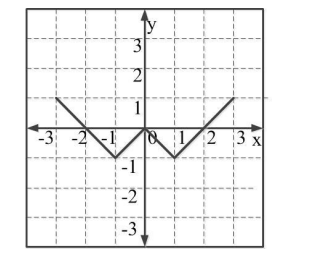
\includegraphics[width=0.5\textwidth]{figures/9.png}
\end{center}
\begin{enumerate}
    \item[(A)] \( y = ||x| + 1| - 2 \)  
    \item[(B)] \( y = ||x| - 1| - 1 \)  
    \item[(C)] \( y = ||x| + 1| - 1 \)  
    \item[(D)] \( y = ||x - 1| - 1| \)  
\end{enumerate}
\vspace{0.5cm}

\questionb{Consider the following three statements: (i) Some roses are red. (ii) All red flowers fade quickly. (iii) Some roses fade quickly. Which of the following statements can be logically inferred from the above statements?}{10}
\begin{enumerate}
    \item[(A)] If (i) is true and (ii) is false, then (iii) is false.  
    \item[(B)] If (i) is true and (ii) is false, then (iii) is true.  
    \item[(C)] If (i) and (ii) are true, then (iii) is true.  
    \item[(D)] If (i) and (ii) are false, then (iii) is false.  
\end{enumerate}
\vspace{0.5cm}

\section*{Technical Section}

\questiona{The Taylor series expansion of the function, \( f(x) = \frac{-1}{1+x} \), around \( x = 0 \) (up to 4\textsuperscript{th} order term) is:}{1}
\begin{enumerate}
    \item[(A)] \( 1 + x + x^2 + x^3 + x^4 \)  
    \item[(B)] \( -1 + x - x^2 + x^3 - x^4 \)  
    \item[(C)] \( -1 - x + x^2 - x^3 + x^4 \)  
    \item[(D)] \( -1 + x - 2x^2 + 3x^3 - 4x^4 \)  
\end{enumerate}
\vspace{0.5cm}

\questiona{The inverse of the matrix \(\begin{bmatrix}1 & 3\\1 & 2\end{bmatrix}\) is,}{2}
\begin{enumerate}
    \item[(A)] \(\begin{bmatrix}2 & 3\\1 & 1\end{bmatrix}\)  
    \item[(B)] \(\begin{bmatrix}-2 & 1\\3 & -1\end{bmatrix}\)  
    \item[(C)] \(\begin{bmatrix}-2 & 3\\1 & -1\end{bmatrix}\)  
    \item[(D)] \(\begin{bmatrix}2 & -3\\-1 & 1\end{bmatrix}\)  
\end{enumerate}
\vspace{0.5cm}

\questiona{The line integral of a vector function \( \vec{F}(\vec{r}) \) over a curve \( C \) in a simply connected domain \( D \) in space, is defined by: \[ \int_C \vec{F}(\vec{r}) \cdot d\vec{r} = \int_C (F_1 dx + F_2 dy + F_3 dz) \] The line integral is independent of path in \( D \). \( F_1, F_2, \) and \( F_3 \) are continuous, and have continuous first partial derivatives in \( D \). \( C' \) is a closed curve in \( D \). Which one of the following is NOT ALWAYS true in domain \( D \)?}{3}
\begin{enumerate}
    \item[(A)] \( \nabla \times \vec{F} = \vec{0} \)  
    \item[(B)] \( \nabla \cdot \vec{F} = 0 \)  
    \item[(C)] \( \oint_{C'} \vec{F}(\vec{r}) \cdot d\vec{r} = 0 \)  
    \item[(D)] \( \vec{F} \times \vec{F} = \vec{0} \)  
\end{enumerate}
\vspace{0.5cm}

\questiona{Which one of the following is the integrating factor (IF) for the differential equation, \( \cos^2 x \frac{dy}{dx} + y = \cos x \)?}{4}
\begin{enumerate}
    \item[(A)] \( e^{\tan x} \)  
    \item[(B)] \( e^{\cos x} \)  
    \item[(C)] \( e^{-\tan x} \)  
    \item[(D)] \( e^{\sin x} \)  
\end{enumerate}
\vspace{0.5cm}

\questiona{A phase diagram of a black oil is shown in the figure (Y is the critical point). Match the following: (P) Curve XY, (Q) Curve YZ, (R) Phase I, (S) Phase II \\ (I) Dew point curve, (II) Single phase liquid, (III) Bubble point curve, (IV) Single phase gas}{5}
\begin{center}
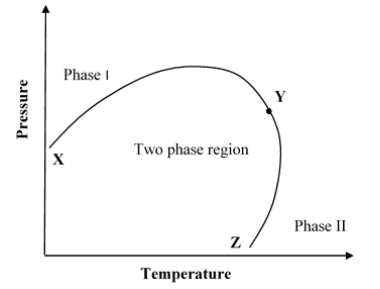
\includegraphics[width=0.5\textwidth]{figures/5.png}
\end{center}
\begin{enumerate}
    \item[(A)] P-I, Q-III, R-II, S-IV  
    \item[(B)] P-III, Q-I, R-II, S-IV  
    \item[(C)] P-III, Q-I, R-IV, S-II  
    \item[(D)] P-I, Q-II, R-III, S-IV  
\end{enumerate}
\vspace{0.5cm}

\questiona{Match the following chemicals to their respective oilfield applications: (P) Hydrate inhibitor, (Q) Well stimulation, (R) Drilling fluid biocide, (S) Viscosifier \\ (I) Formaldehyde, (II) Xanthan gum, (III) Methanol, (IV) Hydrochloric acid}{6}
\begin{enumerate}
    \item[(A)] P-IV, Q-III, R-II, S-I  
    \item[(B)] P-III, Q-I, R-IV, S-II  
    \item[(C)] P-I, Q-III, R-IV, S-II  
    \item[(D)] P-III, Q-IV, R-I, S-II  
\end{enumerate}
\vspace{0.5cm}

\questiona{The CH\textsubscript{4}-hydrate equilibrium curve (dashed) and CO\textsubscript{2}-hydrate equilibrium curve (solid) on a pressure-temperature plane above 0°C are shown in the figure. The two curves divide the plane into four non-overlapping regions. In which region are CO\textsubscript{2}-hydrates stable and CH\textsubscript{4}-hydrates unstable?}{7}
\begin{center}
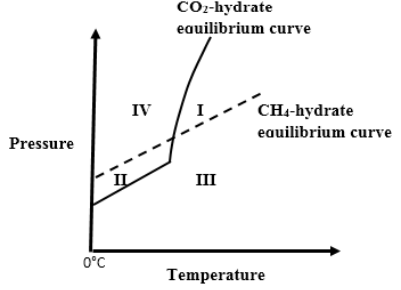
\includegraphics[width=0.5\textwidth]{figures/7.png}
\end{center}
\begin{enumerate}
    \item[(A)] I  
    \item[(B)] II  
    \item[(C)] III  
    \item[(D)] IV  
\end{enumerate}
\vspace{0.5cm}

\questiona{Plot of ratio of pressure to gas compressibility factor (P/Z) vs. cumulative gas production (Gp) for a gas reservoir (represented by solid curve in the figure) was shown to a reservoir engineering student. The student made the following statements: (I) A water aquifer is attached to this gas reservoir. (II) P/Z vs. Gp curve must always be a straight line for water encroachment in a gas reservoir. (III) The ultimate gas recovery is diminished due to water encroachment. Which of the above statements are TRUE?}{8}
\begin{center}
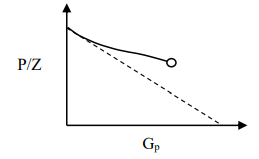
\includegraphics[width=0.5\textwidth]{figures/8.png}
\end{center}
\begin{enumerate}
    \item[(A)] Only I and II  
    \item[(B)] Only II and III  
    \item[(C)] Only I and III  
    \item[(D)] I, II, and III  
\end{enumerate}
\vspace{0.5cm}

\questiona{Waste water from oil industry consists of oil in free and emulsified forms. The oil in the free form can be recovered by:}{9}
\begin{enumerate}
    \item[(A)] Aerated lagoons  
    \item[(B)] Trickling filters  
    \item[(C)] Gravity separators  
    \item[(D)] Biological oxygen pond  
\end{enumerate}
\vspace{0.5cm}

\questiona{A reservoir model consisting of two porous matrices M and N, separated by a fracture, is shown in the figure. The matrices are strongly water-wet and are saturated with oil of specific gravity 0.8. Water is injected only in the fracture at injection well A. If the Reynolds number for the flow in the fracture conduit is assumed to be less than unity, which one of the following forces will dominate oil recovery from the porous matrix M during the water-flood operation?}{10}
\begin{center}
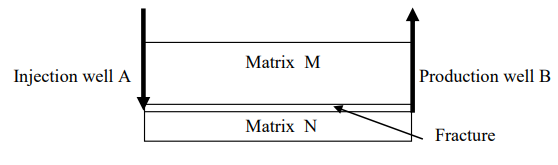
\includegraphics[width=0.5\textwidth]{figures/10.png}
\end{center}
\begin{enumerate}
    \item[(A)] Capillary force  
    \item[(B)] Gravity force  
    \item[(C)] Viscous force  
    \item[(D)] Inertial force  
\end{enumerate}
\vspace{0.5cm}

\questiona{A fractional flow curve is given for a core for which the irreducible water saturation is 0.2 and the residual oil saturation is 0.3. The initial water saturation in the core is 0.3. If Welge’s method is applied to find the breakthrough saturation and fractional flow of water at breakthrough, which point should be used in the figure to draw a tangent line to the fractional flow curve.}{11}
\begin{center}
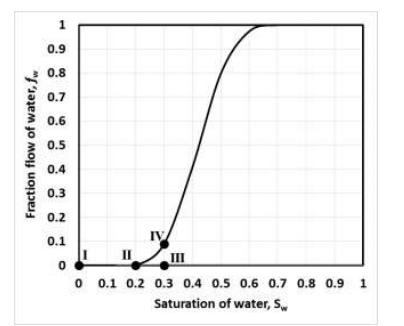
\includegraphics[width=0.5\textwidth]{figures/11.png}
\end{center}
\begin{enumerate}
    \item[(A)] I  
    \item[(B)] II  
    \item[(C)] III  
    \item[(D)] IV  
\end{enumerate}
\vspace{0.5cm}

\questiona{Which one of the following curves represents behavior of oil phase viscosity as a function of pressure in the reservoir (where, \( P_b \) is the bubble point pressure of oil)?}{12}
\begin{center}
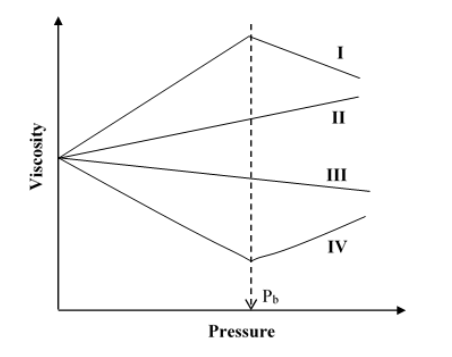
\includegraphics[width=0.5\textwidth]{figures/12.png}
\end{center}
\begin{enumerate}
    \item[(A)] Curve I  
    \item[(B)] Curve II  
    \item[(C)] Curve III  
    \item[(D)] Curve IV  
\end{enumerate}
\vspace{0.5cm}

\questiona{Pick out the INCORRECT statement.}{13}
\begin{enumerate}
    \item[(A)] Flash point is always lower than fire point.  
    \item[(B)] Pour point of lube oil can be reduced by removing the wax from it.  
    \item[(C)] Fracturing is a well stimulation technique.  
    \item[(D)] Coal bed methane typically contains more than 60\% CO\(_2\).  
\end{enumerate}
\vspace{0.5cm}

\questiona{Which one of the following phenomena encountered during flooding is desirable for increasing oil recovery from a reservoir?}{14}
\begin{enumerate}
    \item[(A)] Viscous fingering  
    \item[(B)] Formation damage  
    \item[(C)] Increase in mobility ratio  
    \item[(D)] Decrease in capillary pressure  
\end{enumerate}
\vspace{0.5cm}

\questiona{CO\(_2\) foams are used for enhanced oil recovery due to which of the following reasons? \\ 
(I) It can be used for CO\(_2\) sequestration \\
(II) CO\(_2\) can exist in the form of a dense fluid at reservoir conditions \\
(III) CO\(_2\) can convert to hydrocarbon at the reservoir temperature and pressure \\
(IV) Solubility of CO\(_2\) in oil is higher compared to gases like N\(_2\)}{15}
\begin{enumerate}
    \item[(A)] Only I, II, and III  
    \item[(B)] Only I, II, and IV  
    \item[(C)] Only II, III, and IV  
    \item[(D)] Only I, III, and IV  
\end{enumerate}
\vspace{0.5cm}

\questiona{Which one of the following is FALSE about a typical offshore deepwater oil spill?}{16}
\begin{enumerate}
    \item[(A)] Using boom boats to prevent spilled oil from spreading  
    \item[(B)] Allowing the spill to reach the shore before clearing  
    \item[(C)] Burning of spilled oil  
    \item[(D)] Using a skimmer to collect the oil  
\end{enumerate}
\vspace{0.5cm}

\questiona{Which one of these methods is NOT commonly used to deal with the problem of soil contamination by oil spillage?}{17}
\begin{enumerate}
    \item[(A)] Biodegradation  
    \item[(B)] Leaching out the oil  
    \item[(C)] Soil recycling  
    \item[(D)] Using rain water to wash the contaminants  
\end{enumerate}
\vspace{0.5cm}

\questiona{The factor on which the selection of an offshore platform for the reservoir does NOT depend:}{18}
\begin{enumerate}
    \item[(A)] Water depth  
    \item[(B)] Reservoir fluid properties  
    \item[(C)] Sea bed conditions  
    \item[(D)] Best case weather forecast  
\end{enumerate}
\vspace{0.5cm}

\questiona{Which one of the following options is correct about the effects of steam stimulation in increasing the oil production rate? \\
(I) Reduces the oil viscosity \\
(II) Increases the formation damage \\
(III) Reduces the interfacial tension \\
(IV) Increases the oil viscosity}{19}
\begin{enumerate}
    \item[(A)] Only I and II  
    \item[(B)] Only II and III  
    \item[(C)] Only III and IV  
    \item[(D)] Only I and III  
\end{enumerate}
\vspace{0.5cm}

\questiona{Which one of the following is INCORRECT about oil based drilling muds?}{20}
\begin{enumerate}
    \item[(A)] Good rheological properties at higher temperatures (as high as 250°C)  
    \item[(B)] Effective against corrosion  
    \item[(C)] Detection of gas kick is difficult  
    \item[(D)] Less inhibitive than water based muds  
\end{enumerate}
\vspace{0.5cm}

\questiona{Assume that viscous, gravity, and capillary are the only dominant forces for fluid flow in a given reservoir, a cone formed around the perforation zone will break into the well, when}{21}
\begin{enumerate}
    \item[(A)] capillary forces are more than viscous and gravity forces.  
    \item[(B)] viscous forces are more than gravity forces.  
    \item[(C)] gravity forces are more than capillary forces.  
    \item[(D)] viscous and gravity forces are equal.  
\end{enumerate}
\vspace{0.5cm}

\questiona{Two complex numbers, \( \tilde{z} \) and \( \tilde{\varepsilon} \), are related as follows: \[ \tilde{z} = \frac{\tilde{\varepsilon}}{i\omega} \] where, \( i = \sqrt{-1} \) and \( \omega \) is a scalar. Given principal argument of \( \tilde{\varepsilon} \), \( \text{Arg}(\tilde{\varepsilon}) = -\frac{2\pi}{3} \), the principal argument of \( \tilde{z} \), \( \text{Arg}(\tilde{z}) \) = \underline{\hspace{3cm}} (rounded-off to two decimal places. Use \( \pi = 3.14 \)).}{22}
\vspace{0.5cm}

\questiona{A cylindrical sandstone core, 7.5 cm long and 3.5 cm diameter has grain density of 3 g/cm\(^3\). If the mass of the dry core is 200 g, the porosity of the core is \underline{\hspace{3cm}}\% (rounded-off to two decimal places).}{23}
\vspace{0.5cm}

\questiona{In an oil reservoir the current average pressure is below bubble point pressure of the oil. The current oil production rate is 103 m\(^3\)/day and total gas production rate is 105 m\(^3\)/day at STP conditions (25°C and 1 atm). The formation volume factor of the oil is \( \frac{1.2 \text{ m}^3 \text{ at reservoir pressure}}{\text{m}^3 \text{ at STP}} \) and that of gas is \( \frac{0.01 \text{ m}^3 \text{ at reservoir pressure}}{\text{m}^3 \text{ at STP}} \). The dissolved gas oil ratio is \( \frac{10 \text{ m}^3 \text{ of gas at STP}}{\text{m}^3 \text{ of oil at STP}} \). \\ The gas flow rate at bottom-hole conditions is \underline{\hspace{3cm}} × 10\(^2\) m\(^3\)/day. (rounded-off to two decimal places)}{24}
\vspace{0.5cm}

\questiona{Exponential decline curve is to be used to estimate the oil reserves of a well. The current oil production rate is 1000 m\(^3\)/day and yearly decline rate is 6\% per year. If the minimum oil flow rate economically sustainable for the well is 1 m\(^3\)/day, the reserves (economically producible) associated with the well are \underline{\hspace{3cm}} × 10\(^6\) m\(^3\). (rounded-off to two decimal places. Use 1 year = 365 days)}{25}
\vspace{0.5cm}

\questionb{The probability density for three binomial distributions (D1, D2, and D3) is plotted against number of successful trials in the given figure. Each of the plotted distributions corresponds to a unique pair of (n, p) values, where, n is the number of trials and p is the probability of success in a trial. Three sets of (n, p) values are provided in the table. Set (n, p): I (60, 0.3), II (60, 0.2), III (24, 0.5). Pick the correct match between the (n, p) set and the plotted distribution.}{26}
\begin{center}
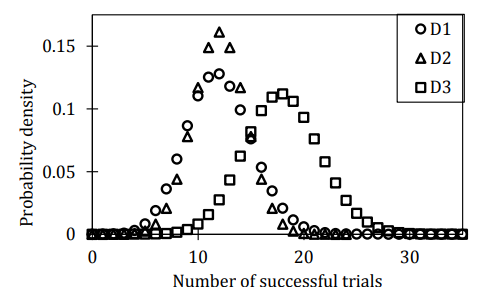
\includegraphics[width=0.5\textwidth]{figures/26.png}
\end{center}
\begin{enumerate}
    \item[(A)] Set I – D1, Set II – D2, Set III – D3  
    \item[(B)] Set I – D3, Set II – D1, Set III – D2  
    \item[(C)] Set I – D2, Set II – D3, Set III – D1  
    \item[(D)] Set I – D2, Set II – D1, Set III – D3  
\end{enumerate}
\vspace{0.5cm}

\questionb{Which of the following statements are true about Natural Gas Hydrates? \\
Natural gas hydrates: \\
(I) are formed under low temperature and high pressure. \\
(II) can store approximately 160 m\(^3\) of gas per m\(^3\) of hydrate at 25°C and 1 atm. \\
(III) formation is an endothermic process. \\
(IV) are potential sources of methane.}{27}
\begin{enumerate}
    \item[(A)] Only II, III \& IV  
    \item[(B)] Only I, II \& III  
    \item[(C)] Only I, II \& IV  
    \item[(D)] Only I, III \& IV  
\end{enumerate}
\vspace{0.5cm}

\questionb{Pwf (bottom-hole well flowing pressure) vs. Q (flow rate) plots show the inflow performance relation (IPR) and vertical lift performance (VLP) curves. Figure I shows VLP curves for two well head pressures \( P_{hw1} \) and \( P_{hw2} \). Figure II shows VLP curves for two well diameters D1 and D2. Which one of the following statements is true?}{28}
\begin{center}
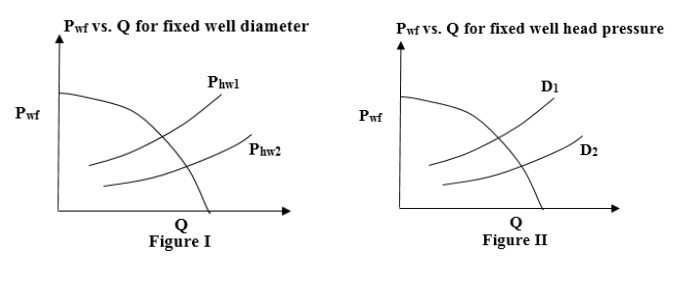
\includegraphics[width=0.5\textwidth]{figures/28.png}
\end{center}
\begin{enumerate}
    \item[(A)] \( P_{hw1} > P_{hw2} \) and \( D_1 < D_2 \)  
    \item[(B)] \( P_{hw1} > P_{hw2} \) and \( D_1 > D_2 \)  
    \item[(C)] \( P_{hw1} < P_{hw2} \) and \( D_1 < D_2 \)  
    \item[(D)] \( P_{hw1} < P_{hw2} \) and \( D_1 > D_2 \)  
\end{enumerate}
\vspace{0.5cm}

\questionb{Match the following: \\
(P) Weber Number (Q) Froude Number (R) Reynolds number (S) Nusselt number \\
(I) Ratio of inertial force to viscous force \\
(II) Ratio of convective heat transfer to conductive heat transfer \\
(III) Ratio of inertial force to interfacial force \\
(IV) Ratio of inertial force to gravitational force}{29}
\begin{enumerate}
    \item[(A)] P-III, Q-IV, R-I, S-II  
    \item[(B)] P-III, Q-II, R-I, S-IV  
    \item[(C)] P-II, Q-III, R-IV, S-I  
    \item[(D)] P-IV, Q-III, R-I, S-II  
\end{enumerate}
\vspace{0.5cm}

\questionb{A dilute mixture of coal and sand particles, both of diameter 100 µm and densities 1800 kg/m\(^3\) and 2600 kg/m\(^3\), respectively, is to be classified by elutriation technique using water (density 1000 kg/m\(^3\), viscosity 10\(^{-3}\) Pa.s). Assuming Stokes law is applicable, the minimum settling velocity of the particles in the mixture is (g = 9.81 m/s\(^2\)):}{30}
\begin{enumerate}
    \item[(A)] \( 4.36 \times 10^{-3} \) m/s  
    \item[(B)] \( 8.72 \times 10^{-3} \) m/s  
    \item[(C)] \( 2.18 \times 10^{-3} \) m/s  
    \item[(D)] \( 1.29 \times 10^{-3} \) m/s  
\end{enumerate}
\vspace{0.5cm}

\questionb{Oil flow rate and flowing bottom-hole pressure (FBHP) recorded with time during a multi-rate well test are shown. Let \( k \) be the reservoir permeability, \( h \) be the formation thickness, and \( \mu \) be the viscosity of the oil. \( \Delta P_D(t) \) is constant-rate dimensionless pressure drop as a function of time. The total pressure drop till time, \( t \), where \( t > t_1 \), will be:}{31}
\begin{center}
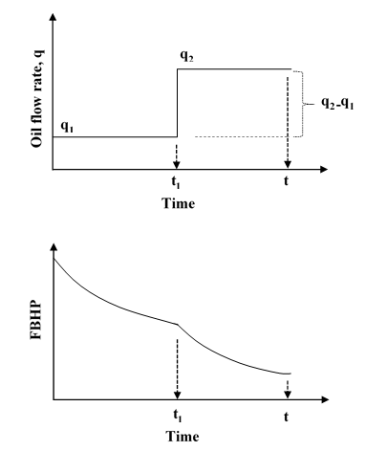
\includegraphics[width=0.5\textwidth]{figures/31.png}
\end{center}
\begin{enumerate}
    \item[(A)] \( \frac{q_1 \mu}{2\pi k h} \Delta P_D(t) + \frac{(q_2 - q_1)\mu}{2\pi k h} \Delta P_D(t - t_1) \)  
    \item[(B)] \( \frac{q_1 \mu}{2\pi k h} \Delta P_D(t_1) + \frac{(q_2 - q_1)\mu}{2\pi k h} \Delta P_D(t - t_1) \)  
    \item[(C)] \( \frac{q_1 \mu}{2\pi k h} \Delta P_D(t) + \frac{q_2 \mu}{2\pi k h} \Delta P_D(t - t_1) \)  
    \item[(D)] \( \frac{q_1 \mu}{2\pi k h} \Delta P_D(t_1) + \frac{q_2 \mu}{2\pi k h} \Delta P_D(t) \)  
\end{enumerate}
\vspace{0.5cm}

\questionb{Which one of the following options presents the correct combination? \\
(P) Reservoir limit test \hspace{0.5cm} (I) Communication between wells \\
(Q) Modified isochronal test \hspace{0.5cm} (II) Ideally zero flowing bottom hole pressure \\
(R) Interference test \hspace{1.6cm} (III) Extended drawdown test \\
(S) Absolute open flow potential \hspace{0.35cm} (IV) Drawdown and build-up test of equal duration}{32}
\begin{enumerate}
    \item[(A)] P-II, Q-III, R-I, S-IV  
    \item[(B)] P-IV, Q-I, R-III, S-II  
    \item[(C)] P-III, Q-IV, R-I, S-II  
    \item[(D)] P-I, Q-III, R-IV, S-II  
\end{enumerate}
\vspace{0.5cm}

\questionb{Which one of the following options presents the correct combination? \\
(P) Roller Cone bits \hspace{1.5cm} (I) Long and widely spaced teeth \\
(Q) PDC bits \hspace{2.7cm} (II) Journal (Pin) angle \\
(R) Soft formation \hspace{2.0cm} (III) Short and wider teeth \\
(S) Hard formation \hspace{1.6cm} (IV) Size of the cutting \\
(T) Back rake angle \hspace{2.0cm} (V) 1400\(^\circ\)C and 6×10\(^5\) psi}{33}
\begin{enumerate}
    \item[(A)] P-II, Q-V, R-I, S-III, T-IV  
    \item[(B)] P-III, Q-IV, R-I, S-II, T-V  
    \item[(C)] P-III, Q-II, R-IV, S-I, T-V  
    \item[(D)] P-II, Q-V, R-III, S-I, T-IV  
\end{enumerate}
\vspace{0.5cm}

\questionb{Primary and secondary indicators of kick in a well where the indicators are: \\
1) flow rate increase, 2) gas, oil or water-cut muds, 3) pit volume increase, \\
4) flowing well with mud pump shut-off, 5) reduction in drill-pipe weight, 6) drilling break. \\
Which one of the following presents the correct combination?}{34}
\begin{enumerate}
    \item[(A)] Primary (1, 3, 5) and Secondary (2, 4, 6)  
    \item[(B)] Primary (1, 2, 3) and Secondary (4, 5, 6)  
    \item[(C)] Primary (1, 2, 4) and Secondary (3, 5, 6)  
    \item[(D)] Primary (1, 3, 4) and Secondary (2, 5, 6)  
\end{enumerate}
\vspace{0.5cm}

\questionb{Relative permeability curve for the two rock types (X: solid line and Y: dashed line) are shown in the diagram, where \( S_w \) is the fractional water saturation. Which one of the following statements is correct about wettability and consolidated nature of the two rock types?}{35}
\begin{center}
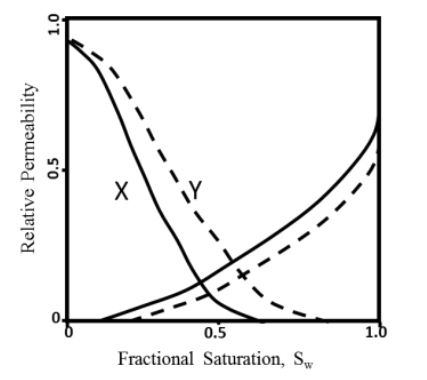
\includegraphics[width=0.5\textwidth]{figures/35.png}
\end{center}
\begin{enumerate}
    \item[(A)] X is more consolidated and mixed wet, Y is less consolidated and water wet  
    \item[(B)] X is more consolidated and water wet, Y is less consolidated and mixed wet  
    \item[(C)] X is less consolidated and mixed wet, Y is more consolidated and water wet  
    \item[(D)] X is less consolidated and water wet, Y is more consolidated and mixed wet  
\end{enumerate}
\vspace{0.5cm}

\questionb{Which one of the following options presents correct combinations of exploration methods with their respective frequency of operation? \\
(P) Seismic \hspace{2cm} (I) ~10\(^6\) Hz \\
(Q) Sonic \hspace{2.2cm} (II) ~10\(^2\) Hz \\
(R) Controlled Source EM \hspace{0.5cm} (III) ~10\(^4\) Hz \\
(S) Ultrasonic \hspace{1.5cm} (IV) ~1 Hz}{36}
\begin{enumerate}
    \item[(A)] P-IV, Q-II, R-I, S-III  
    \item[(B)] P-II, Q-III, R-IV, S-I  
    \item[(C)] P-II, Q-I, R-IV, S-III  
    \item[(D)] P-IV, Q-I, R-II, S-III  
\end{enumerate}
\vspace{0.5cm}

\questionb{Which one of the following options presents the correct combinations? \\
(P) Borisov’s \hspace{2cm} (I) Critical rate correlation in vertical wells with coning \\
(Q) Schols’ \hspace{2.3cm} (II) Horizontal well performance relation \\
(R) Efros’ \hspace{2.5cm} (III) Vertical well performance relation \\
(S) Wiggins’ \hspace{2cm} (IV) Critical rate correlation in horizontal wells with coning}{37}
\begin{enumerate}
    \item[(A)] P-II, Q-IV, R-I, S-III  
    \item[(B)] P-IV, Q-III, R-II, S-I  
    \item[(C)] P-IV, Q-II, R-III, S-I  
    \item[(D)] P-II, Q-I, R-IV, S-III  
\end{enumerate}
\vspace{0.5cm}

\questionb{Which one of the following options represents the typical sequence of applying cut-offs for pay zone identification in a conventional reservoir?}{38}
\begin{enumerate}
    \item[(A)] porosity, saturation, shale  
    \item[(B)] porosity, permeability, saturation  
    \item[(C)] shale, porosity, saturation  
    \item[(D)] shale, porosity, permeability  
\end{enumerate}
\vspace{0.5cm}

\questionb{Which one of the following options represents the correct sequence of arrival of acoustic wave energy recorded in a sonic log?}{39}
\begin{enumerate}
    \item[(A)] shear, surface, compressional  
    \item[(B)] compressional, shear, surface  
    \item[(C)] surface, shear, compressional  
    \item[(D)] compressional, surface, shear  
\end{enumerate}
\vspace{0.5cm}

\questionb{The variation of the amount of salt in a tank with time is given by, \[ \frac{dx}{dt} + 0.025x = 20 \] where, \( x \) is the amount of salt in kg and \( t \) is the time in minutes. Given that there is no salt in the tank initially, the time at which the amount of salt increases to 200 kg is \underline{\hspace{3cm}} minutes. (rounded-off to two decimal places)}{40}
\vspace{0.5cm}

\questionb{Solve the given differential equation using the 2nd order Runge-Kutta (RK2) method: \[ \frac{dy}{dt} = t - \sqrt{y} \] \\
Initial condition: \( y(t=0) = 4 \) \\
Use the following form of RK2 method with an integration step-size, \( h = 0.5 \): \\
\( k_1 = f(t_i, y_i) \), \( k_2 = f(t_i + 0.5h, y_i + 0.5k_1 h) \), \( y_{i+1} = y_i + k_2 h \) \\
The value of \( y(t = 0.5) = \underline{\hspace{3cm}} \). (rounded-off to two decimal places)}{41}
\vspace{0.5cm}

\questionb{A box contains 100 balls of same size, of which, 25 are black and 75 are white. Out of 25 black balls, 5 have a red dot. A trial consists of randomly picking a ball and putting it back in the same box, i.e., sampling is done with replacement. Two such trials are done. \\
The conditional probability that no black ball with a red dot is picked given that at least one black ball is picked, is \underline{\hspace{3cm}}. (in fraction rounded-off to two decimal places)}{42}
\vspace{0.5cm}

\questionb{A cylindrical pipeline of length 30 km is transporting naphtha. Pressure sensors are attached along pipe length to detect leaks. Under steady-state, leak-free operation, there is a linear pressure drop along the length (z) of the pipeline. If a leak occurs, the pressure profile develops a kink at the leak point \( z_{\text{leak}} \). \\
Assume that there is only one leak-point (4 km < \( z_{\text{leak}} \) < 27 km) and a new steady-state is reached. The steady-state pressure measurements at four locations along the pipe-length are provided in the table. The location of the leak-point using the gradient intersection method is \underline{\hspace{3cm}} km. (rounded-off to two decimal places)}{43}
\begin{center}
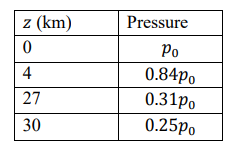
\includegraphics[width=0.3\textwidth]{figures/43.png}
\end{center}
\vspace{0.5cm}

\questionb{A dry core was subjected to the mercury injection test in the laboratory. Following are the related details: \\
Average formation porosity = 0.2, Formation volume factor, \( B_O = 1.2 \) reservoir-bbl/STB \\
Oil API\(_o\) = 32, Specific gravity of water = 1.1 \\
Hydrostatic gradient = 0.433 psi/ft \\
\( (\sigma_{OW} \cos \theta)_{\text{res}} = 26 \) dyne/cm, \( (\sigma_{AM} \cos \theta)_{\text{lab}} = 367 \) dyne/cm \\
Average drainage area = 80 acres, (1 acre-ft = 7758 bbl) \\
The table shows the laboratory data for capillary pressure at different mercury saturations. \\
\begin{tabular}{|c|c|}
\hline
\( P_c \) (psia) & Mercury saturation (S\textsubscript{Hg}) \\
\hline
10 & 0.0075 \\
17 & 0.25 \\
30 & 0.50 \\
108 & 0.70 \\
2000 & 0.85 \\
\hline
\end{tabular} \\
\( P_c = \frac{2\sigma \cos \theta}{r} \), and the average water saturation (\( S_W \)) for the productive column is 0.25. The Original Oil in Place (OOIP) in the productive column where \( S_W \leq 0.5 \) is \underline{\hspace{3cm}} MMSTB. (rounded-off to one decimal place)}{44}
\vspace{0.5cm}

\questionb{A well is drilled with water based mud. The water saturation in the completely flushed zone (no formation fluid residual) is given by, \[
S_{xo} = \left( \frac{a}{\phi^2} \cdot \frac{R_{mf}}{R_{xo}} \right)^{1/2}
\] where, \( R_{mf} \) and \( R_{xo} \) are the mud filtrate resistivity and flushed zone resistivity, respectively. Use, \( a = 1.0 \) and \( R_{xo} = 25 R_{mf} \). \\
The calculated porosity (\( \phi \)) of the formation is \underline{\hspace{3cm}}. (in fraction rounded-off to two decimal places)}{45}
\vspace{0.5cm}

\questionb{An oil well is tested at a flow rate (Q) of 50 BOPD. The bottom hole flowing pressure (P\textsubscript{wf}) is 500 psia. The shut-in pressure is 1000 psia. If P\textsubscript{wf} is lowered to 300 psia and assuming the Vogel’s correlation holds, the estimated flow rate in the oil well is \underline{\hspace{3cm}} BOPD (rounded-off to two decimal places). \\
The Vogel’s correlation is: \[
\frac{Q}{Q_{\text{max}}} = 1 - 0.2\left( \frac{P_{wf}}{\bar{P}} \right) - 0.8\left( \frac{P_{wf}}{\bar{P}} \right)^2
\]}{46}
\vspace{0.5cm}

\questionb{Using Miller, Dyes and Hutchinson (MDH) method, the skin factor of an oil well is found to be \( s = -3.5 \). \\
The reservoir and fluid properties are: \\
Formation porosity is 0.20, Total compressibility is \( 2.5 \times 10^{-5} \) psia\(^{-1} \), Oil viscosity is 1.5 cP, Wellbore radius is 0.5 ft \\
Flowing bottom hole pressure at \( \Delta t = 0 \) is 2830 psia, Shut-in pressure at \( \Delta t = 1 \) hr is 3000 psia \\
Slope of middle time region (MTR) line in MDH plot is 190 psia/cycle \\
The permeability of the reservoir is \underline{\hspace{3cm}} mD. (rounded-off to two decimal places)}{47}
\vspace{0.5cm}

\questionb{An oil well (producing under expansion drive only) in a reservoir is subjected to two pressure build-up tests. The average formation thickness of the reservoir is 13 ft, the total compressibility is \( 1 \times 10^{-5} \) psia\(^{-1} \), and porosity is 0.2. The average formation volume factor of oil is 1.3 reservoir-bbl/STB. Average reservoir pressure during the first test and the second test was found to be 3500 psia and 3200 psia, respectively. \\
If the oil produced between the two pressure build-up tests in 180 days is 250 STB/day, the area of the reservoir is \underline{\hspace{3cm}} acres. (rounded-off to two decimal places)}{48}
\vspace{0.5cm}

\questionb{A well in a very large reservoir has a wellbore radius of 10 cm. The sandstone, with a porosity of 0.25 and 12\% (by grain volume) calcite (CaCO\(_3\)), is to be acidized with a preflush (HCl solution) so as to dissolve all the calcite up to a distance of 1 m from the wellbore. 1 m\(^3\) of preflush is able to dissolve 0.082 m\(^3\) CaCO\(_3\). Assume that the reaction between HCl and CaCO\(_3\) is instantaneous. \\
The minimum preflush volume required per meter of the formation thickness is \underline{\hspace{3cm}} m\(^3\). (rounded-off to two decimal places)}{49}
\vspace{0.5cm}

\questionb{At a particular temperature, the vapour pressure of benzene and toluene are 4 atm and 1.2 atm, respectively. The composition of the liquid at equilibrium is 0.5 moles of benzene and 0.5 moles of toluene. Assuming ideal gas and ideal solution, the equilibrium vapour phase mole fraction of benzene is \underline{\hspace{3cm}}. (rounded-off to two decimal places)}{50}
\vspace{0.5cm}

\questionb{Saturated steam at 0.7 atm and 90°C condenses on a vertical pipe of 2 cm outside diameter and 40 cm length. The average condensation heat transfer coefficient on the tube is 12000 W/m\(^2\)K. The outside surface temperature of the pipe is maintained constant at 85°C. The enthalpy values for saturated steam and condensate are 2660 kJ/kg and 375 kJ/kg, respectively. \\
The rate of steam condensation is \underline{\hspace{3cm}} kg/h. (rounded-off to two decimal places)}{51}
\vspace{0.5cm}

\questionb{Oil is being transported between two reservoirs with the help of three parallel pipes at steady state. The diameters of these pipes are 2 cm, 3 cm and 4 cm, respectively. The pipes are equal in length and the flow is laminar. The discharge through the 4 cm diameter pipe is 50 liters/s. \\
The discharge through the 2 cm diameter pipe is \underline{\hspace{3cm}} liters/s. (rounded-off to two decimal places)}{52}
\vspace{0.5cm}

\questionb{A driller finds an oil reservoir with a gas cap starting at a depth of 1000 m from the surface. The gas-oil contact was found at 1100 m depth and water-oil contact was found at 1300 m depth. The water pressure in the aquifer below the oil zone varies with depth from the surface (h, in meters) as, \( P = h \times 10^4 \) Pa. The density of the oil is 900 kg/m\(^3\) and that of the gas is 5 kg/m\(^3\) at the reservoir condition. \\
The minimum density of the mud needed to stop the gas kick when the driller reaches at the top of the gas cap is \underline{\hspace{3cm}} kg/m\(^3\). (rounded-off to two decimal places. Use \( g = 9.81 \) m/s\(^2\))}{53}
\vspace{0.5cm}

\questionb{The viscosity, \( \mu \) (in Pa.s) of a power law fluid as a function of shear rate, \( \dot{\gamma} \) (in s\(^{-1}\)) is given by the following relation: \[
\mu = \frac{1}{2} |\dot{\gamma}|^{-1}
\] This power law fluid lies between two infinitely large horizontal parallel plates separated by a distance (h) of \( 10^{-3} \) m. The top plate is moving horizontally at a velocity (v) of \( 10^{-3} \) m/s and the bottom plate is held stationary. Assuming laminar flow and neglecting gravity, the absolute value of steady-state shear stress acting on the bottom plate is \underline{\hspace{3cm}} Pa. (rounded-off to two decimal places)}{54}
\vspace{0.5cm}

\questionb{A heterogeneous rectangular rock of cross-sectional area 1 m\(^2\) perpendicular to the flow is being flooded by water to measure the effective permeability from cross-section AA’ to cross-section CC’. \\
The pressure at the cross-sections AA’, BB’, and CC’ is 2 bar, 1.5 bar, and 1 bar, respectively. The permeability in milli-Darcy and lengths AB and BC in meters are given in the figure. The effective permeability of the rock from AA’ to CC’ is \underline{\hspace{3cm}} mD. (rounded-off to two decimal places)}{55}
\begin{center}
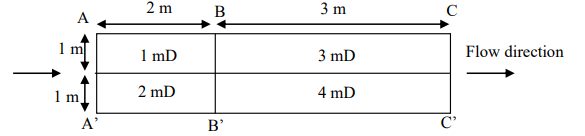
\includegraphics[width=0.7\textwidth]{figures/55.png}
\end{center}
\vspace{0.5cm}

\vspace{5cm}
\begin{center}
\textbf{END OF THE QUESTION PAPER} \\
\rule{\textwidth}{0.5pt}
\end{center}

\end{document}
